\section{Auswertung}
\label{sec:Auswertung}

\subsection{Bestimmung des spezifischen Widerstandes}
Die Dicke des Kupferdrahtes ist $d_{DK}=\qty{0.104(0.001)}{\milli\meter}$ und die des Silberdrahtes ist $d_{DS}=\qty{0.263(0.001)}{\milli\meter}$.
Mit 
\begin{equation}
  A=\pi \bigl(\frac{d}{2} \bigr)^2
\label{eqn:Querschnitt}
\end{equation}
\noindent 
kann dann die Fläche $A_{DK}=\qty{0.00849(0.00016)}{\milli\meter\squared}$ und $A_{DS}=\qty{0.0543(0.0004)}{\milli\meter\squared}$.
\noindent Für die Kupferspule, bei der die Länge des Drahtes $L_K=\qty{1.37}{\meter}$ ist, und für die Silberspule mit $L_S=\qty{1.73}{\meter}$, wird außerdem der ohmsche Widerstand gemessen.
Dieser beträgt $R_K=\qty{2.7050}{\ohm}$ und $R_S=\qty{0.6086}{\ohm}$.

\noindent Jetzt kann mit der Formel \ref{eqn:} der spezifische Widerstand von Kupfer und Silber bestimmt werden.


\noindent Für Kupfer beträgt dieser $\varrho_K=\qty{0.01677(0.00032)}{\ohm\milli\meter\squared\per\m}$ und für Silber $\varrho_S=\qty{0.00299(0.00006)}{\ohm\milli\meter\squared\per\m}$.

\noindent Bei Zink ist der spezifische Widerstand $\varrho_Z = \qty{0.06}{\ohm\milli\meter\squared\per\m}$ \cite{Zink}.


\subsection{Messung des Hall Effektes}

In den Tabellen \ref{tab:Silber}, \ref{tab:Kupfer} und \ref{tab:Zink} ist für Silber, Kupfer und dann Zink die Hall-Spannung $U_H$ abhängig von der magnetischen Flussdichte $B$ eingetragen.
Die magnetische Flussdichte wird dabei durch eine Änderung der Stromstärke durch die Elektromagneten $I_B$ angepasst.


\begin{table}[H]
  \centering
  \caption{Hier ist die Hall Spannung bei der Silberplatte in Abhängikeit zu $I_B$ und damit zu $B$ aufgeführt.}
  \label{tab:Silber}
  \begin{tblr}{
    colspec={S[table-format=1.1] S[table-format=4.1] S[table-format=1.3]},
    row{1}={guard,mode=math},
  }
  \toprule
  I_B \mathbin{/} \unit{\ampere} & B \mathbin{/} \unit{\milli\tesla} & U_H \mathbin{/} \unit{\milli\volt} \\
  \midrule
  1.0  &    340.0 & 0.161 \\
  1.5  &    513.9 & 0.157 \\
  2.0  &    676.0 & 0.153 \\
  2,5  &    919.6 & 0.149 \\
  3.0  &   1131.0 & 0.145 \\
  3.5  &   1229.7 & 0.142 \\
  4.0  &   1320.0 & 0.139 \\
  \bottomrule
  \end{tblr}
\end{table}

\begin{table}[H]
  \centering
  \caption{Eingetragen ist die Hall-Spannung abhängig von der magnetischen Flussdichte, die von der Stromstärke durch die Elektromagneten $I_B$ abhängt.}
  \label{tab:Kupfer}
  \begin{tblr}{
    colspec={S[table-format=1.2] S[table-format=4.1] S[table-format=2.3]},
    row{1}={guard,mode=math},
  }
  \toprule
  I_B \mathbin{/} \unit{\ampere} & B \mathbin{/} \unit{\milli\tesla} & U_H \mathbin{/} \unit{\milli\volt} \\
  \midrule
  1.00   &  350.3 &  0.000 \\
  1.50   &  516.9 & -0.003 \\
  2.00   &  674.9 & -0.005 \\
  2.50   &  930.4 & -0.008 \\
  3.00   & 1134.3 & -0.010 \\
  3.50   & 1147.4 & -0.015 \\
  0.75   & 1729.0 & -0.002 \\
  1.25   & 2708.0 & -0.004 \\
  \bottomrule
  \end{tblr}
\end{table}






\begin{table}[H]
  \centering
  \caption{Die Hall-Spannung ist, abghängig von der magnetischen Flussdichte, die mit der Stromstärke durch die Spulen $I_B$ eingestellt wird, aufgetragen.}
  \label{tab:Zink}
  \begin{tblr}{
    colspec={S[table-format=1.2] S[table-format=4.1] S[table-format=1.3]},
    row{1}={guard,mode=math},
  }
  \toprule
  I_B \mathbin{/} \unit{\ampere} & B \mathbin{/} \unit{\milli\tesla} & U_H \mathbin{/} \unit{\milli\volt} \\
  \midrule
  1.00  &   343.0 & 0.341 \\
  1.50  &   514.5 & 0.344 \\
  2.00  &   677.9 & 0.347 \\
  2.50  &   918.0 & 0.352 \\
  3.00  &  1135.7 & 0.352 \\
  0.50  &  1292.3 & 0.333 \\
  1.25  &  2734.5 & 0.335 \\
  \bottomrule
  \end{tblr}
\end{table}

\noindent In \ref{fig:plot} wird für alle drei Metalle die Hall-Spannung gegen die magnetische FLussdichte aufgetragen.
Dabei ist die Reihenfolge von links nach rechts: Silber, Kupfer und dann Zink.

\begin{figure}
  \centering
  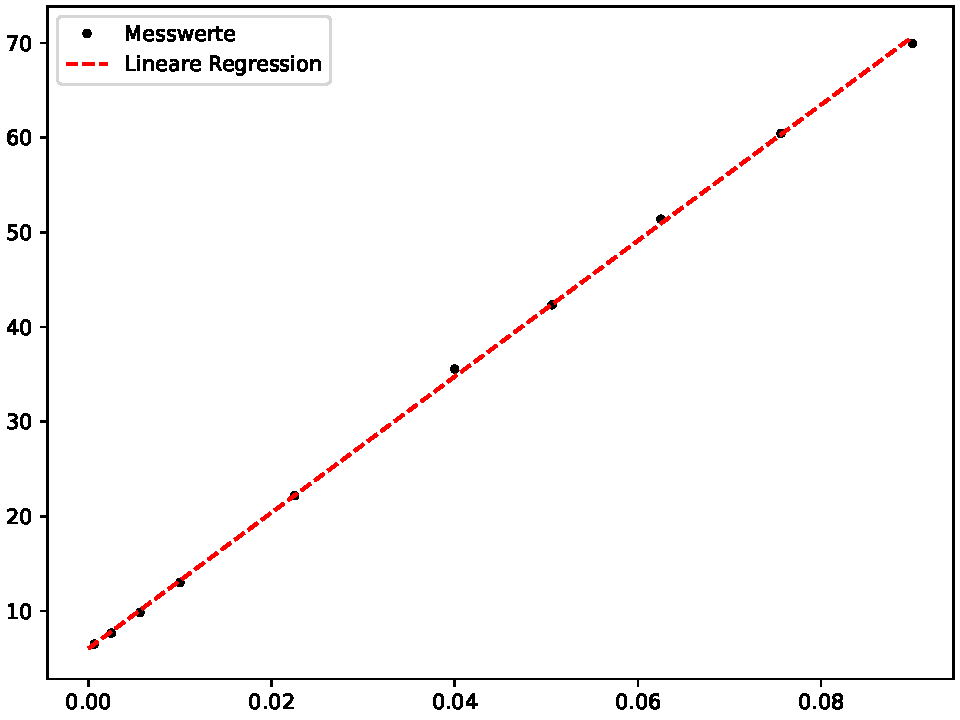
\includegraphics{plot.pdf}
  \caption{Hier wird für Silber, Kupfer und Zink die gemessene Hall-Spannung gegen die magnetische Flussdichte aufgetragen. Zudem wurde eine Regressionsgerade eingefügt.}
  \label{fig:plot}
\end{figure}

\noindent Die Steigung der Regressionsgeraden ist dabei das Verhältnis von Hall-Spannunng zur magnetischen Flussdichte.
Damit beträgt dieses Verhältnis $V=\Bigl(\frac{U_H}{B}\Bigr)$ bei Silber \\ $V_S=\qty{-2.1312(0.0802)e-05}{\volt\per\tesla}$, bei Kupfer
 $V_K=\qty{-1.5418(0.2417)e-05}{\volt\per\tesla}$ und bei Zink $V_Z=\qty{1.4943(0.2223)e-05}{\volt\per\tesla} $.


